\documentclass[10pt, a4paper,spanish]{article}

\usepackage[utf8]{inputenc}
\usepackage[spanish]{babel}

\usepackage[T1]{fontenc}

\usepackage[hmarginratio=1:1,top=32mm,columnsep=20pt]{geometry}
\usepackage[hang, small,labelfont=bf,up,textfont=it,up]{caption}


\usepackage{graphicx}
\graphicspath{ {images/} }

\usepackage{titlesec}
\renewcommand\thesection{\Roman{section}}
\renewcommand\thesubsection{\Roman{subsection}}
\titleformat{\section}[block]{\large\scshape\centering}{\thesection.}{1em}{}
\titleformat{\subsection}[block]{\large}{\thesubsection.}{1em}{}

\usepackage{fancyhdr}
\pagestyle{fancy}
\fancyhead{}
\fancyfoot{}
\fancyhead[C]{ \today \ $\bullet$ Minería de Datos $\bullet$ Lógica y Representación del Conocimiento}
\fancyfoot[RO]{\thepage}

%-------------------------------------------------------------------------------
%	TITLE SECTION
%-------------------------------------------------------------------------------

\title{\vspace{-15mm}\fontsize{24pt}{10pt}\selectfont\textbf{Lógica y Representación del Conocimiento}} % Article title

\author{Sergio García Prado}
\date{\today}

%-------------------------------------------------------------------------------

\begin{document}

	\maketitle % Insert title

	\thispagestyle{fancy} % All pages have headers and footers

%-------------------------------------------------------------------------------
%	TEXT
%-------------------------------------------------------------------------------

	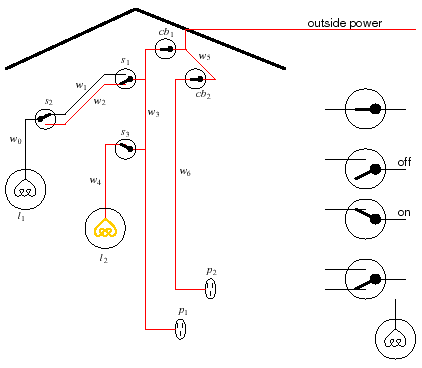
\includegraphics[width=0.9\textwidth]{diagnostic-assistant}

	\section{Elaborar una base de conocimiento para el asistente al diagnóstico en el dominio del cableado de una vivienda. Las reglas generales deben de permitir codificar la instancia específica que muestra la figura. Utilizar los principios generales para la elaboración de una ontología específica.}

		\paragraph{}


	\section{Partiendo de la base de conocimiento del asistente al diagnóstico que hemos utilizado en las prácticas de la asignatura, elaborar la ontología que la soporta. Compararla con la ontología elaborada en el problema anterior.}

		\paragraph{}



\end{document}
